\section{1184006 - Murnia Lestari}
\subsection{Teori}
\begin{enumerate}

	\item Jelaskan apa itu binary classification dilengkapi ilustrasi gambar sendiri.
	\hfill\break
merupakan sebuah metode atau konsep dasar yang mengklasifikasikan elemen-elemen himpunan menjadi dua kelompok berdasarkan aturan klasifikasi yang sudah ditentukan. Contohnya seperti gambar dibawah ini :

	\begin{figure}[h]
	\centering
		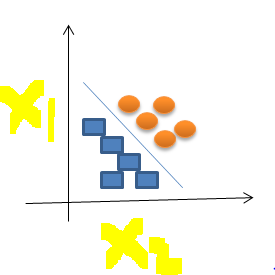
\includegraphics[width=4cm]{figures/1184006/chapter2/1.PNG}
		\caption{Binary classification.}
	\end{figure}

	\item Jelaskan apa itu supervised learning dan unsupervised learning dan clustering dengan ilustrasi gambar sendiri.
	\hfill\break

	\begin{itemize}
		\item Supervised Learning
		\hfill\break merupakan algoritma mesin yang memiliki attribut tambahan seperti x dan y yang ingin diprediksi. Contohnya seperti gambar dibawah ini :
		
		\begin{figure}[h]
		\centering
			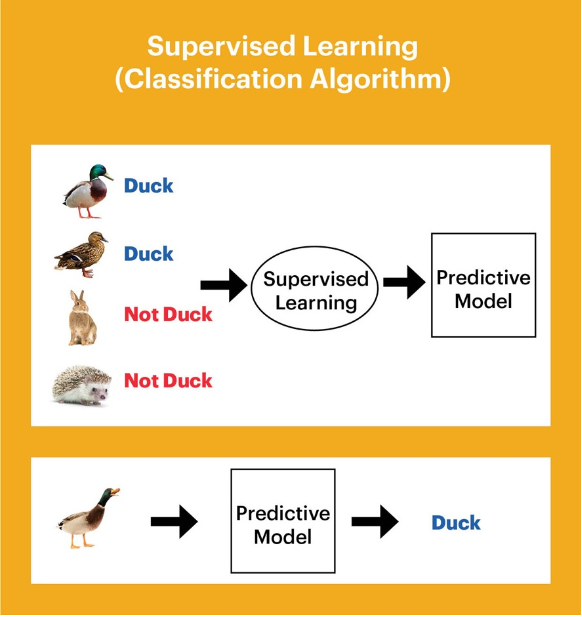
\includegraphics[width=6cm]{figures/1184006/chapter2/2.PNG}
			\caption{Supervised Learning.}
		\end{figure}

		\newpage\item Unsupervised Learning 
		\hfill\break
		Berbeda dengan Supervised Learning, Unsupervised Learning  merupakan algoritma yang tidak memiliki attribut tambahan yang akan diprediksi melainkan dengan melihat kesamaan dari dari attrribut-attribut yang dimiliki. Contohnya seperti gambar dibawah ini :


		\begin{figure}[h]
		\centering
			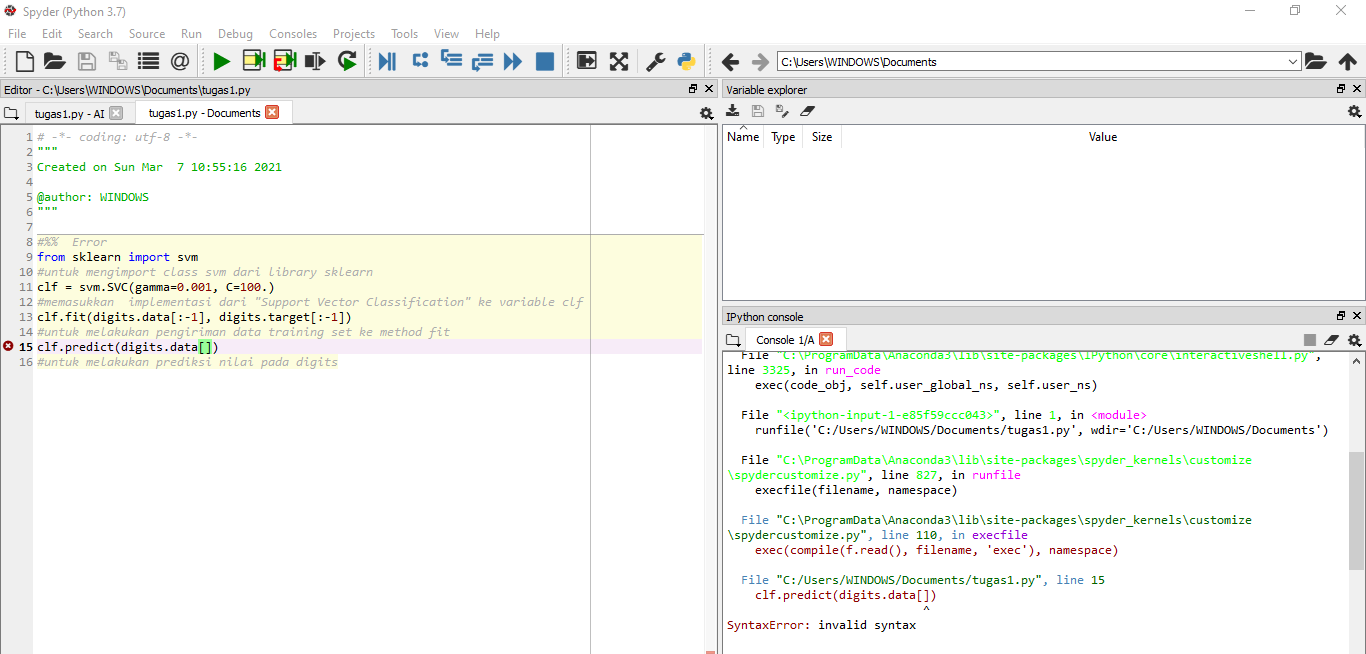
\includegraphics[width=6cm]{figures/1184006/chapter2/3.PNG}
			\caption{Unsupervised Learning.}
		\end{figure}

		\item Clustering
		\hfill\break
		Clustering adalah sebuah metode yang mengelompokan  objek yang tampaknya sama dalam kelompok  ojek yang sama (disebut cluster) lebih mirip (dalam beberapa kasus) satu sama lain daripada kelompok lain (cluster). Contohnya seperti gambar dibawah ini :
		\begin{figure}[h]
		\centering
			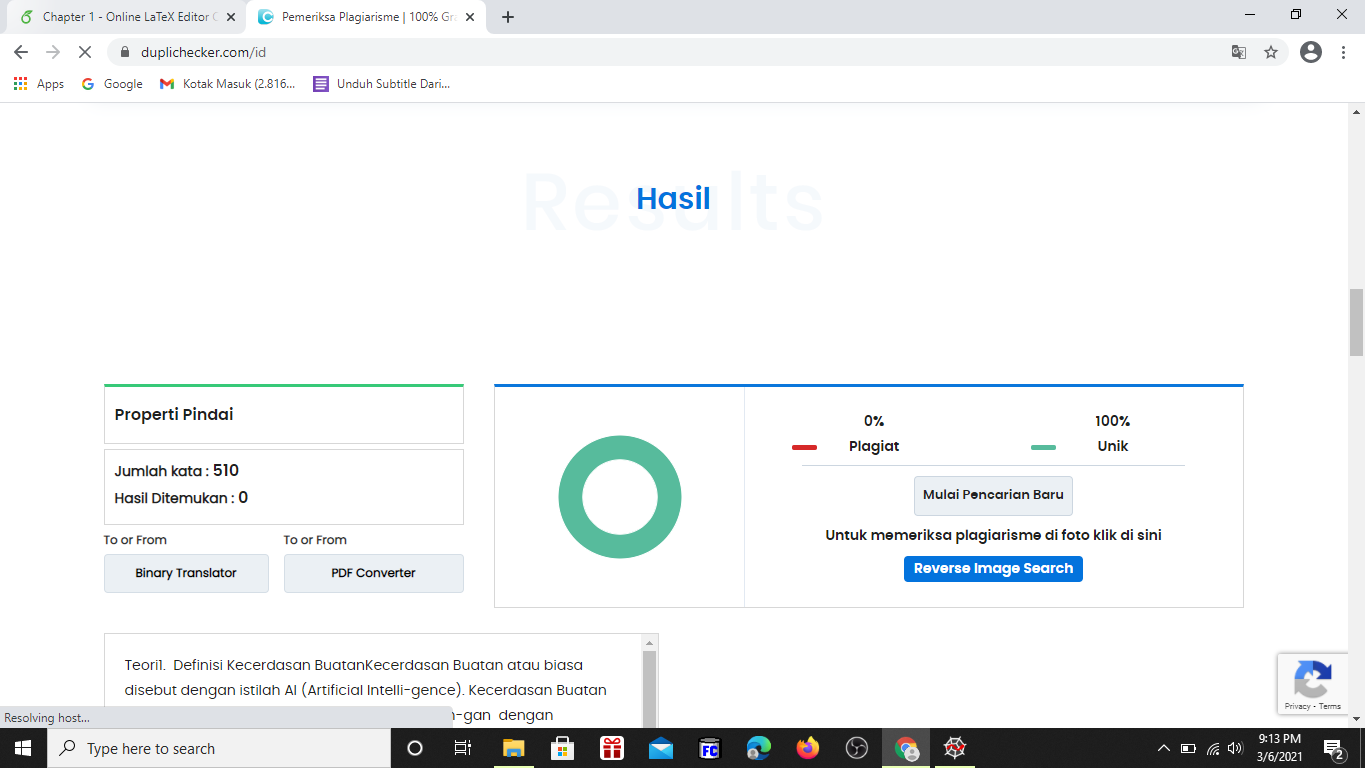
\includegraphics[width=6cm]{figures/1184006/chapter2/4.PNG}
			\caption{Clustering.}
		\end{figure}
	\end{itemize}
	
	\item Jelaskan apa itu evaluasi dan akurasi dari buku dan disertai ilustrasi contoh dengan gambar sendiri.
	\hfill\break
	Evaluasi merupakan sebuah metode evaluasi yang mengukur tingkat akurasinya. Sedangkan Akurasi merupakan tingkat persentase dari pembelajaran yang dievaluasi. Berikut merupakan contoh dari  evaluasi dan clustering.
	\begin{figure}[h]
	\centering
		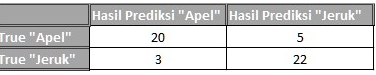
\includegraphics[width=10cm]{figures/1184006/chapter2/5.PNG}
		\caption{Evaluasi dan Akurasi.}
	\end{figure}

	\item Jelaskan bagaimana cara membuat dan membaca confusion matrix, buat confusion matrix buatan sendiri.
	\hfill\break
	\begin{enumerate}
	\item Cara membuat dan membaca confusion matrix :
	\begin{itemize}
	\item Tentukan pokok permasalahan dan atributanya, misal gaji dan listrik.
	\item Buat pohon keputusan
	\item Lalu data testingnya
	\item Lalu mencari nilai a, b, c, dan d. Semisal a = 5, b = 1, c = 1, dan d = 3.
	\item Selanjutnya mencari nilai recall, precision, accuracy, serta dan error rate.
	\end{itemize}
	\item Berikut adalah contoh dari confusion matrix :
	\begin{itemize}
	\item Recall =3/(3+3) = 0,5
	\item Precision = 3/(3+5) = 0,375
	\item Accuracy =(3+5)/(3+5+5+3) = 0,5
	\end{itemize}
	\end{enumerate}

	\begin{figure}[h]
	\centering
		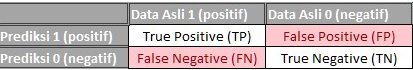
\includegraphics[width=7cm]{figures/1184006/chapter2/6.PNG}
		\caption{Confusion Matrix.}
	\end{figure}

	\item Jelaskan bagaimana K-fold cross validation bekerja dengan gambar ilustrasi contoh buatan sendiri.
	\hfill\break
	\begin{itemize}
	\item Total instance dibagi menjadi N bagian.
	\item Fold yang pertama adalah bagian pertama menjadi data uji (testing data) dan sisanya menjadi training data.
	\item Lalu hitung akurasi berdasarkan porsi data tersebut dengan menggunakan persamaan.
	\item Fold yang ke dua adalah bagian ke dua menjadi data uji (testing data) dan sisanya training data. 
	\item Kemudian hitung akurasi berdasarkan porsi data tersebut.
	\item Dan seterusnya hingga habis mencapai fold ke-K.
	\item Terakhir hitung rata-rata akurasi K buah.
	\end{itemize}

	\begin{figure}[h]
	\centering
		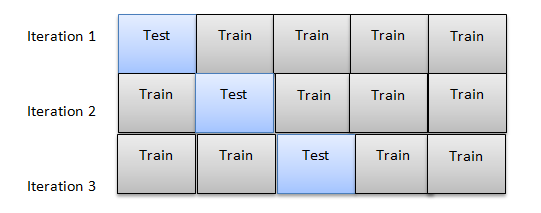
\includegraphics[width=7cm]{figures/1184006/chapter2/7.PNG}
		\caption{K-fold Cross Validation.}
	\end{figure}

	\item Jelaskan apa itu decision tree dengan gambar ilustrasi contoh buatan sendiri.
	\hfill\break
	Decision tree atau pohon keputusan merupakan metode klasifikasi yang digunakan untuk memprediksi dengan mengunakan struktur pohon atau struktur hierarki.

	\begin{figure}[h]
	\centering
		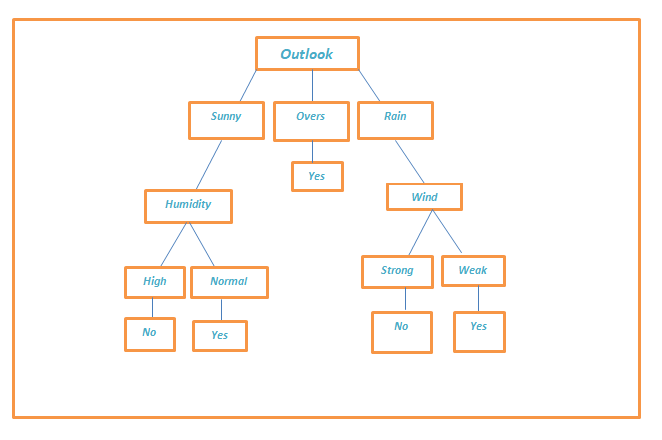
\includegraphics[width=9cm]{figures/1184006/chapter2/8.PNG}
		\caption{Decision Tree.}
	\end{figure}

	\item Jelaskan apa itu information gain dan entropi dengan gambar ilustrasi buatan sendiri.
	\hfill\break
	Information gain merupakan sebuah metode yang menggunakan teknik scoring untuk memberikan bobot yang ada  pada sebuah fitur dengan memaksimalkan entropy. Sedangka entropi merupakan  ukuran yang yang dibaca dalam informasi gain yang sedang diproses. Semakin tinggi entropi, semakin sulit untuk menarik kesimpulan dari informasi itu. Membalik koin adalah contoh tindakan yang memberikan informasi acak. Untuk koin yang tidak memiliki afinitas terhadap kepala atau ekor, hasil lemparannya sulit diprediksi. Mengapa Karena tidak ada hubungan antara yang menentang dan hasil. Inilah inti dari entropi.
	\begin{figure}[h]
	\centering
		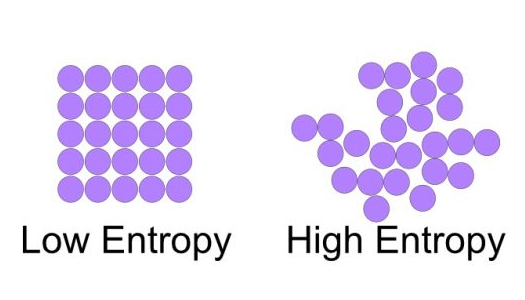
\includegraphics[width=6cm]{figures/1184006/chapter2/9.PNG}
		\caption{Entropi.}
	\end{figure}


\end{enumerate}


\subsection{Praktek}
\begin{enumerate}
	\item Soal 1
	\hfill\break
	\lstinputlisting[firstline=8, lastline=20]{src/1184006/chapter2/1184006.py}
	Kode di atas digunakan untuk mengimpor atau mengirim library pandas sebagai pd. Kemudian ditentukan variabel "apel" untuk dipanggil dataset diperoleh dari data student-mat.csv. Hasilnya adalah sebagai berikut :
	\begin{figure}[h]
	\centering
		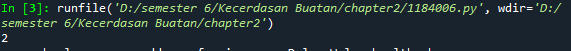
\includegraphics[width=4cm]{figures/1184006/chapter2/1-m.PNG}
		\caption{Hasil Soal 1.}
	\end{figure}
	\item Soal 2
	\hfill\break
	\lstinputlisting[firstline=21, lastline=33]{src/1184006/chapter2/1184006.py}
	Kode di atas ada bagian mendeklarasikan pass/fail nya data berdasarkan G1+G2+G3. Dengan ketentuan nilai pass nya yaitu sama dengan 30. kemudian pada variabel medan dideklarasikan jika baris dengan G1+G2+G3 ditambahkan, dan hasilnya sama dengan 35 maka axisnya 1. Hasilnya adalah sebagai berikut :
	\begin{figure}[h]
	\centering
		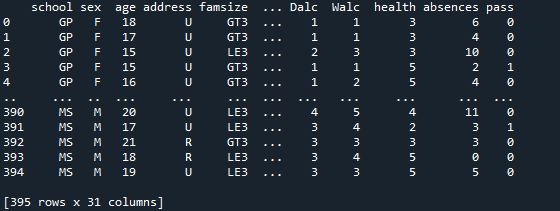
\includegraphics[width=4cm]{figures/1184006/chapter2/2-m.PNG}
		\caption{Hasil Soal 2.}
	\end{figure}
	\item Soal 3
	\hfill\break
	\lstinputlisting[firstline=34, lastline=41]{src/1184006/chapter2/1184006.py}
	One-hot encoding adalah proses di mana variabel kategorikal dikonversi menjadi bentuk yang dapat disediakan untuk algoritma ML untuk melakukan pekerjaan yang lebih baik dalam prediksi. Metode head ini digunakan untuk mengembalikan baris n atas 5 secara default dari frame atau seri data Karena saya memuat data menggunakan. Hasilnya adalah sebagai berikut :
	\begin{figure}[h]
	\centering
		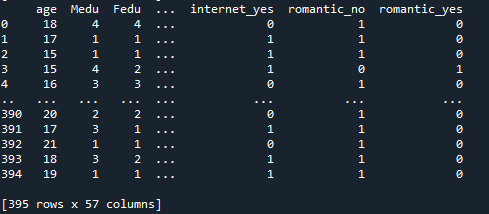
\includegraphics[width=4cm]{figures/1184006/chapter2/3-m.PNG}
		\caption{Hasil Soal 3.}
	\end{figure}
	\item Soal 4
	\hfill\break
	\lstinputlisting[firstline=42, lastline=70]{src/1184006/chapter2/1184006.py}
	Sample digunakan untuk mengembalikan sampel acak item dari objek. Pada bagian tersebut, terdapat train dan test yaing digunakan untuk untuk membagi train, test dan kemudian membagi lagi train ke validasi dan test. Kemudia akan mengimport module numpy sebagai np yang akan digunakan untuk mengembalikan nilai passing dari pelajar dari keseluruhan dataset dengan cara print. Hasilnya adalah sebagai berikut :
	\begin{figure}[h]
	\centering
		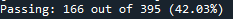
\includegraphics[width=4cm]{figures/1184006/chapter2/4-m.PNG}
		\caption{Hasil Soal 4.}
	\end{figure}
	\item Soal 5
	\hfill\break
	\lstinputlisting[firstline=72, lastline=81]{src/1184006/chapter2/1184006.py}
	Dari librari scikitlearn import modul tree. Kemudian definisikan variabel asahan dengan menggunakan DecisionClassifier. Kemudian pada variabel asahan terdapat Criterion yaitu suatu fungsi untuk mengukur kualitas split, setelah itu agar DecisionTreeClassifier dapat dijalankan gunakan perintah fit. Hasilnya adalah sebagai berikut :
	\begin{figure}[h]
	\centering
		
\includegraphics[width=5cm]{figures/1184006/chapter2/5-m.PNG}
		\caption{Hasil Soal 5.}
	\end{figure}
\item Soal 6
	\hfill\break
	\lstinputlisting[firstline=82, lastline=92]{src/1184006/chapter2/1184006.py}
	Graphviz adalah perangkat lunak visualisasi grafik open source. Visualisasi grafik adalah cara mewakili informasi struktural sebagai diagram grafik dan jaringan abstrak. Hasilnya adalah sebagai berikut :
	\begin{figure}[h]
	\centering
		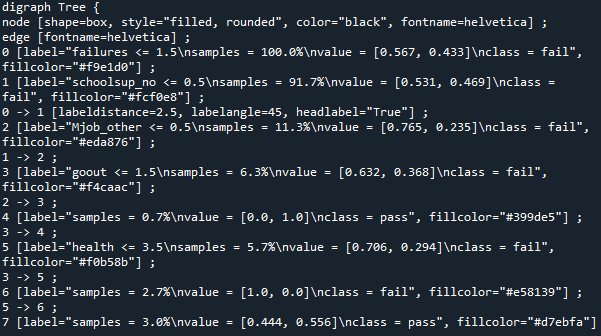
\includegraphics[width=4cm]{figures/1184006/chapter2/6-m.PNG}
		\caption{Hasil Soal 6.}
	\end{figure}
	\item Soal 7
	\hfill\break
	\lstinputlisting[firstline=93, lastline=96]{src/1184006/chapter2/1184006.py}
	Tree.export graphviz merupakan fungsi yang menghasilkan representasi Graphviz dari decision tree, yang kemudian ditulis ke outfile.Disini akan menyimpan classifiernya, akan meng ekspor file student performance jika salah akan mengembalikan nilai fail. 

	\item Soal 8
	\hfill\break
	\lstinputlisting[firstline=98, lastline=100]{src/1184006/chapter2/1184006.py}
	Score juga disebut prediksi, dan merupakan proses menghasilkan nilai berdasarkan model pembelajaran mesin yang terlatih, diberi beberapa data input baru. Nilai atau skor yang dibuat dapat mewakili prediksi nilai masa depan, tetapi mereka juga mungkin mewakili kategori atau hasil yang mungkin. Jadi disini asahan akan memprediksi nilai dari medan test att dan test pass .
\item Soal 9
	\hfill\break
	\lstinputlisting[firstline=101, lastline=109]{src/1184006/chapter2/1184006.py}
	Skrip ini akan mengevaluasi score dengan validasi silang. Dimana variabel scores berisikan crossvalscore yang merupakan fungsi pembantu pada estimator dan dataset. Kemudian akan menampilkan score rata rata dan kurang lebih dua standar deviasi yang mencakup 95 persen score. 
	\item Soal 10
	\hfill\break
	\lstinputlisting[firstline=111, lastline=119]{src/1184006/chapter2/1184006.py}
	Pada skrip ini menunjukkan seberapa dalam tree itu. Semakin dalam tree, semakin banyak perpecahan yang dimilikinya dan menangkap lebih banyak informasi tentang data. variabel asahan akan mendefinisikan tree nya yang kemudian variabel scores akan mengevaluasi score dengan validasi silang. disini mendefinisikan decision tree dengan kedalaman mulai dari 1 hingga 20. Hasilnya adalah sebagai berikut :
	\begin{figure}[h]
	\centering
		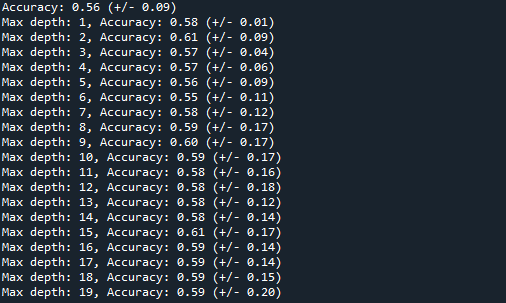
\includegraphics[width=4cm]{figures/1184006/chapter2/10-m.PNG}
		\caption{Hasil Soal 10.}
	\end{figure}
\item Soal 11
	\hfill\break
	\lstinputlisting[firstline=121, lastline=144]{src/1184006/chapter2/1184006.py}
	Depth acc akan membuat array kosong dengan mengembalikan array baru dengan bentuk dan tipe yang diberikan, tanpa menginisialisasi entri. Dengan 19 sebagai bentuk array kosong, 3 sebagai output data-type dan float urutan kolomutama (gaya Fortran) dalam memori. variabel asahan yang akan melakukan split score akan mengvalidasi score secara silang. Hasilnya adalah sebagai berikut :
	\begin{figure}[h]
	\centering
		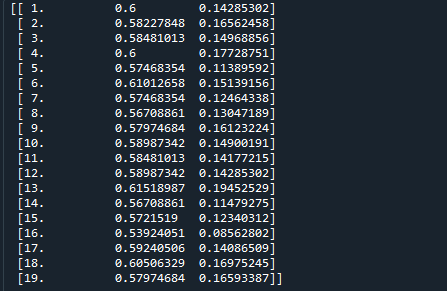
\includegraphics[width=4cm]{figures/1184006/chapter2/11-m.PNG}
		\caption{Hasil Soal 11.}
	\end{figure}
	\item Soal 12
	\hfill\break
	\lstinputlisting[firstline=145, lastline=153]{src/1184006/chapter2/1184006.py}
	Mengimpor librari dari matplotlib yaitu pylot sebagai plt fig dan ax menggunakan subplots untuk membuat gambar dan satu set subplot. axerrorbar akan membuat error bar kemudian grafik akan ditampilkan menggunakan show. Hasilnya adalah sebagai berikut :
	\begin{figure}
	\centering
		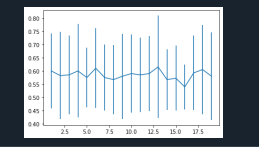
\includegraphics[width=10cm]{figures/1184006/chapter2/12-m.PNG}
		\caption{Hasil Soal 12.}
	\end{figure}
\end{enumerate}
\newpage\subsection{Penanganan Error}
\begin{enumerate}
	\item ScreenShoot Error
	\begin{figure}[h]
		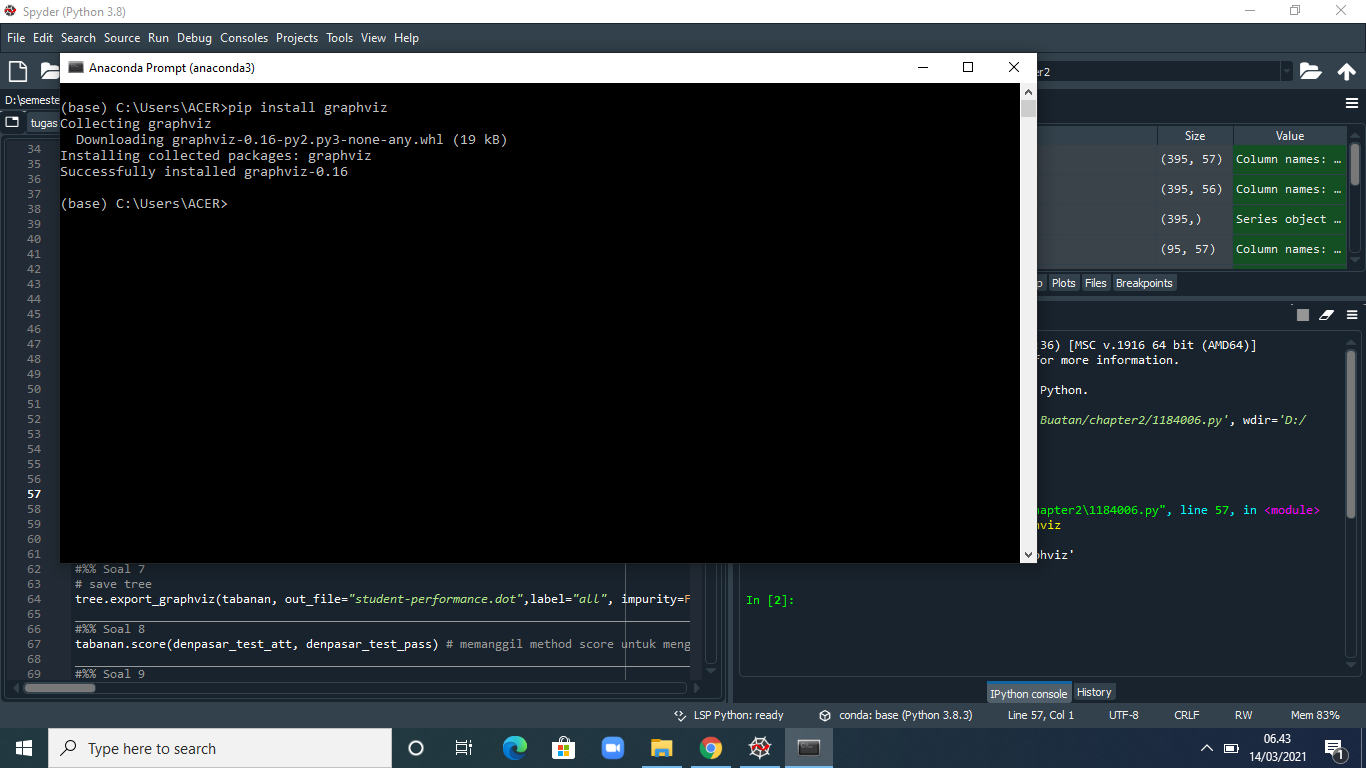
\includegraphics[width=10cm]{figures/1184006/chapter2/eror1.png}
		\centering
		\caption{ModuleNotFoundError}
	\end{figure}
	\item Tuliskan Kode Error dan Jenis Error
	\begin{itemize}
	\lstinputlisting[firstline=82, lastline=92]{src/1184006/chapter2/1184006.py}
		\item ModuleNotFoundError
	\end{itemize}
	\item Cara Penangan Error
	\begin{itemize}
		\item ModuleNotFoundError
		\hfill\break
		Error terdapat pada kesalahan modul graphviz yang belum di install, solusinya ialah menginstall library tersebut di anaconda.
	\end{itemize}
\end{enumerate}
